\documentclass[aspectratio=169]{beamer}\usepackage[]{graphicx}\usepackage[]{xcolor}
% maxwidth is the original width if it is less than linewidth
% otherwise use linewidth (to make sure the graphics do not exceed the margin)
\makeatletter
\def\maxwidth{ %
  \ifdim\Gin@nat@width>\linewidth
    \linewidth
  \else
    \Gin@nat@width
  \fi
}
\makeatother

\definecolor{fgcolor}{rgb}{0.345, 0.345, 0.345}
\newcommand{\hlnum}[1]{\textcolor[rgb]{0.686,0.059,0.569}{#1}}%
\newcommand{\hlsng}[1]{\textcolor[rgb]{0.192,0.494,0.8}{#1}}%
\newcommand{\hlcom}[1]{\textcolor[rgb]{0.678,0.584,0.686}{\textit{#1}}}%
\newcommand{\hlopt}[1]{\textcolor[rgb]{0,0,0}{#1}}%
\newcommand{\hldef}[1]{\textcolor[rgb]{0.345,0.345,0.345}{#1}}%
\newcommand{\hlkwa}[1]{\textcolor[rgb]{0.161,0.373,0.58}{\textbf{#1}}}%
\newcommand{\hlkwb}[1]{\textcolor[rgb]{0.69,0.353,0.396}{#1}}%
\newcommand{\hlkwc}[1]{\textcolor[rgb]{0.333,0.667,0.333}{#1}}%
\newcommand{\hlkwd}[1]{\textcolor[rgb]{0.737,0.353,0.396}{\textbf{#1}}}%
\let\hlipl\hlkwb

\usepackage{framed}
\makeatletter
\newenvironment{kframe}{%
 \def\at@end@of@kframe{}%
 \ifinner\ifhmode%
  \def\at@end@of@kframe{\end{minipage}}%
  \begin{minipage}{\columnwidth}%
 \fi\fi%
 \def\FrameCommand##1{\hskip\@totalleftmargin \hskip-\fboxsep
 \colorbox{shadecolor}{##1}\hskip-\fboxsep
     % There is no \\@totalrightmargin, so:
     \hskip-\linewidth \hskip-\@totalleftmargin \hskip\columnwidth}%
 \MakeFramed {\advance\hsize-\width
   \@totalleftmargin\z@ \linewidth\hsize
   \@setminipage}}%
 {\par\unskip\endMakeFramed%
 \at@end@of@kframe}
\makeatother

\definecolor{shadecolor}{rgb}{.97, .97, .97}
\definecolor{messagecolor}{rgb}{0, 0, 0}
\definecolor{warningcolor}{rgb}{1, 0, 1}
\definecolor{errorcolor}{rgb}{1, 0, 0}
\newenvironment{knitrout}{}{} % an empty environment to be redefined in TeX

\usepackage{alltt}

% Set lecture number for later use


% Part common to all the lectures
\subtitle{MATH 8xyz -- Lecture 02}
\author{\texorpdfstring{Julien Arino\newline Department of Mathematics @ University of Manitoba \newline Maud Menten Institute @ PIMS\newline\url{julien.arino@umanitoba.ca}}{Julien Arino}}
\date{Winter 20XX}

% Title of the lecture
\title{Epidemiology and mathematical epidemiology}



\usetheme{default}
% Slide setup, colour independent

\usepackage{amsmath,amssymb,amsthm}
\usepackage[utf8]{inputenc}
\usepackage{colortbl}
\usepackage{bm}
\usepackage{xcolor}
\usepackage{dsfont}
\usepackage{setspace}
% To use \ding{234} and the like
\usepackage{pifont}
% To cross reference between slide files
\usepackage{zref-xr,zref-user}
% Use something like
% \zexternaldocument{fileI}
% in the tex files. And cite using \zref instead of \ref
\usepackage{booktabs}
\usepackage{marvosym}
\usepackage{cancel}
%\usepackage{transparent}
% Make doi clickable in the bibliography?
\usepackage{doi}

\usepackage[T1]{fontenc}

\usepackage{longtable}

% For heavier titles
\usepackage{helvet} % Enables Helvetica font family


% Fields and the like
\def\IC{\mathbb{C}}
\def\IE{\mathbb{E}}
\def\IF{\mathbb{F}}
\def\II{\mathbb{I}}
\def\IJ{\mathbb{J}}
\def\IK{\mathbb{K}}
\def\IM{\mathbb{M}}
\def\IN{\mathbb{N}}
\def\IP{\mathbb{P}}
\def\IR{\mathbb{R}}
\newcommand{\IRplus}{\mathbb{R}_{\ge 0}}
\def\IZ{\mathbb{Z}}
\def\11{\mathds{1}}


% Bold lowercase
\def\ba{\bm{a}}
\def\bb{\bm{b}}
\def\bc{\bm{c}}
\def\bd{\bm{d}}
\def\be{\bm{e}}
\def\bf{\bm{f}}
\def\bg{\bm{g}}
\def\bh{\bm{h}}
\def\bi{\bm{i}}
\def\bj{\bm{j}}
\def\bk{\bm{k}}
\def\bn{\bm{n}}
\def\bp{\bm{p}}
\def\br{\bm{r}}
\def\bs{\bm{s}}
\def\bu{\bm{u}}
\def\bv{\bm{v}}
\def\bw{\bm{w}}
\def\bx{\bm{x}}
\def\by{\bm{y}}
\def\bz{\bm{z}}
\newcommand{\vect}[1]{\bm{#1}}

% Bold capitals
\def\bB{\bm{B}}
\def\bD{\bm{D}}
\def\bE{\bm{E}}
\def\bF{\bm{F}}
\def\bG{\bm{G}}
\def\bI{\bm{I}}
\def\bL{\bm{L}}
\def\bN{\bm{N}}
\def\bP{\bm{P}}
\def\bR{\bm{R}}
\def\bS{\bm{S}}
\def\bT{\bm{T}}
\def\bX{\bm{X}}

% Bold numbers
\def\b0{\bm{0}}

% Bold greek
\bmdefine{\bmu}{\bm{\mu}}
\def\bphi{\bm{\phi}}
\def\bvarphi{\bm{\varphi}}
\def\bPi{\bm{\Pi}}
\def\bGamma{\bm{\Gamma}}

% Bold red sentence
\def\boldred#1{{\color{red}\textbf{#1}}}
\def\defword#1{{\color{orange}\textbf{#1}}}

% Caligraphic letters
\def\A{\mathcal{A}}
\def\B{\mathcal{B}}
\def\C{\mathcal{C}}
\def\D{\mathcal{D}}
\def\E{\mathcal{E}}
\def\F{\mathcal{F}}
\def\G{\mathcal{G}}
\def\H{\mathcal{H}}
\def\I{\mathcal{I}}
\def\L{\mathcal{L}}
\def\M{\mathcal{M}}
\def\N{\mathcal{N}}
\def\P{\mathcal{P}}
\def\R{\mathcal{R}}
\def\S{\mathcal{S}}
\def\T{\mathcal{T}}
\def\U{\mathcal{U}}
\def\V{\mathcal{V}}

% Adding space for prime (') where needed
\def\pprime{\,'}
% Adding space for star (\star) where needed
\def\pstar{{\,\star}}

% tt font for code
\def\code#1{{\tt #1}}

% i.e., e.g.
\def\eg{\emph{e.g.}}
\def\ie{\emph{i.e.}}


% Operators and special symbols
\def\nbOne{{\mathchoice {\rm 1\mskip-4mu l} {\rm 1\mskip-4mu l}
{\rm 1\mskip-4.5mu l} {\rm 1\mskip-5mu l}}}
\def\cov{\ensuremath{\mathsf{cov}}}
\def\Var{\ensuremath{\mathsf{Var}\ }}
\def\Im{\textrm{Im}\;}
\def\Re{\textrm{Re}\;}
\def\det{\ensuremath{\mathsf{det}}}
\def\diag{\ensuremath{\mathsf{diag}}}
\def\nullspace{\ensuremath{\mathsf{null}}}
\def\nullity{\ensuremath{\mathsf{nullity}}}
\def\rank{\ensuremath{\mathsf{rank}}}
\def\range{\ensuremath{\mathsf{range}}}
\def\sgn{\ensuremath{\mathsf{sgn}}}
\def\Span{\ensuremath{\mathsf{span}}}
\def\tr{\ensuremath{\mathsf{tr}}}
\def\imply{$\Rightarrow$}
\def\restrictTo#1#2{\left.#1\right|_{#2}}
\newcommand{\parallelsum}{\mathbin{\!/\mkern-5mu/\!}}
\def\dsum{\mathop{\displaystyle \sum }}%
\def\dind#1#2{_{\substack{#1\\ #2}}}

\newcommand{\Qmatrix}[1]{%
  \begin{pmatrix}#1\end{pmatrix}%
}

\DeclareMathOperator{\GL}{GL}
\DeclareMathOperator{\Rel}{Re}
\def\Nt#1{\left|\!\left|\!\left|#1\right|\!\right|\!\right|}
\newcommand{\tripbar}{|\! |\! |}



% The beamer bullet (in base colour)
\def\bbullet{\leavevmode\usebeamertemplate{itemize item}\ }

% Theorems and the like
\newtheorem{proposition}[theorem]{Proposition}
\newtheorem{property}[theorem]{Property}
\newtheorem{importantproperty}[theorem]{Property}
\newtheorem{importanttheorem}[theorem]{Theorem}
%\newtheorem{lemma}[theorem]{Lemma}
%\newtheorem{corollary}[theorem]{Corollary}
\newtheorem{remark}[theorem]{Remark}
\setbeamertemplate{theorems}[numbered]
%\setbeamertemplate{theorems}[ams style]

%
%\usecolortheme{orchid}
%\usecolortheme{orchid}

\def\red{\color[rgb]{1,0,0}}
\def\blue{\color[rgb]{0,0,1}}
\def\green{\color[rgb]{0,1,0}}

% Fix skipping lines after items in the bibliography
\setbeamertemplate{bibliography entry title}{}
\setbeamertemplate{bibliography entry location}{}
\setbeamertemplate{bibliography entry note}{}

% Get rid of navigation stuff
\setbeamertemplate{navigation symbols}{}

% Set footline/header line
\setbeamertemplate{footline}
{%
\quad p. \insertpagenumber \quad--\quad \insertsection\vskip2pt
}
% \setbeamertemplate{headline}
% {%
% \quad\insertsection\hfill p. \insertpagenumber\quad\mbox{}\vskip2pt
% }


\makeatletter
\newlength\beamerleftmargin
\setlength\beamerleftmargin{\Gm@lmargin}
\makeatother

% Colours for special pages
\def\extraContent{yellow!20}


%%%%%%%%%%%%%%%%%
\usepackage{tikz}
\usetikzlibrary{shapes,arrows}
\usetikzlibrary{positioning}
\usetikzlibrary{shapes.symbols,shapes.callouts,patterns}
\usetikzlibrary{calc,fit}
\usetikzlibrary{backgrounds}
\usetikzlibrary{decorations.pathmorphing,fit,petri}
\usetikzlibrary{automata}
\usetikzlibrary{fadings}
\usetikzlibrary{patterns,hobby}
\usetikzlibrary{backgrounds,fit,petri}
\usetikzlibrary{tikzmark}

\usepackage{pgfplots}
\pgfplotsset{compat=1.6}
\pgfplotsset{ticks=none}

\usetikzlibrary{decorations.markings}
\usetikzlibrary{arrows.meta}
\tikzset{>=stealth}

% For tikz
\tikzstyle{cloud} = [draw, ellipse,fill=red!20, node distance=0.87cm,
minimum height=2em]
\tikzstyle{line} = [draw, -latex']


%%% For max frame images
\newenvironment{changemargin}[2]{%
\begin{list}{}{%
\setlength{\topsep}{0pt}%
\setlength{\leftmargin}{#1}%
\setlength{\rightmargin}{#2}%
\setlength{\listparindent}{\parindent}%
\setlength{\itemindent}{\parindent}%
\setlength{\parsep}{\parskip}%
}%
\item[]}{\end{list}}


% Make one image take up the entire slide content area in beamer,.:
% centered/centred full-screen image, with title:
% This uses the whole screen except for the 1cm border around it
% all. 128x96mm
\newcommand{\titledFrameImage}[2]{
\begin{frame}{#1}
%\begin{changemargin}{-1cm}{-1cm}
\begin{center}
\includegraphics[width=108mm,height=\textheight,keepaspectratio]{#2}
\end{center}
%\end{changemargin}
\end{frame}
}

% Make one image take up the entire slide content area in beamer.:
% centered/centred full-screen image, no title:
% This uses the whole screen except for the 1cm border around it
% all. 128x96mm
\newcommand{\plainFrameImage}[1]{
\begin{frame}[plain]
%\begin{changemargin}{-1cm}{-1cm}
\begin{center}
\includegraphics[width=108mm,height=76mm,keepaspectratio]{#1}
\end{center}
%\end{changemargin}
\end{frame}
}

% Make one image take up the entire slide area, including borders, in beamer.:
% centered/centred full-screen image, no title:
% This uses the entire whole screen
\newcommand{\maxFrameImage}[1]{
\begin{frame}[plain]
\begin{changemargin}{-1cm}{-1cm}
\begin{center}
\includegraphics[width=\paperwidth,height=\paperheight,keepaspectratio]
{#1}
\end{center}
\end{changemargin}
\end{frame}
}

% This uses the entire whole screen (to include in frame)
\newcommand{\maxFrameImageNoFrame}[1]{
\begin{changemargin}{-1cm}{-1cm}
\begin{center}
\includegraphics[width=\paperwidth,height=0.99\paperheight,keepaspectratio]
{#1}
\end{center}
\end{changemargin}
}

% Make one image take up the entire slide area, including borders, in beamer.:
% centered/centred full-screen image, no title:
% This uses the entire whole screen
\newcommand{\maxFrameImageColor}[2]{
\begin{frame}[plain]
\setbeamercolor{normal text}{bg=#2!20}
\begin{changemargin}{-1cm}{-1cm}
\begin{center}
\includegraphics[width=\paperwidth,height=\paperheight,keepaspectratio]
{#1}
\end{center}
\end{changemargin}
\end{frame}
}


\usepackage{tikz}
\usetikzlibrary{patterns,hobby}
\usepackage{pgfplots}
\pgfplotsset{compat=1.6}
\pgfplotsset{ticks=none}

\usetikzlibrary{backgrounds}
\usetikzlibrary{decorations.markings}
\usetikzlibrary{arrows.meta}
\tikzset{>=stealth}

\tikzset{
  clockwise arrows/.style={
    postaction={
      decorate,
      decoration={
        markings,
        mark=between positions 0.1 and 0.9 step 40pt with {\arrow{>}},
   }}}}


% Beginning of a section
\newcommand{\newSectionSlide}[1]{
\begin{frame}[noframenumbering,plain]
  \begin{tikzpicture}[remember picture,overlay]
    \node[above right,inner sep=0pt,opacity=0.2] at (current page.south west)
    {
        \includegraphics[height=\paperheight,width=\paperwidth]{#1}
    };
  \end{tikzpicture}
  \setbeamercolor{section in toc}{fg=section_page_list_colour}
  \setbeamerfont{section in toc}{size=\Large,series=\bfseries}
  \setbeamertemplate{section in toc shaded}[default][60]
  \tableofcontents[
    currentsection,
    sectionstyle=show/shaded,
    subsectionstyle=show/hide/hide,
    subsubsectionstyle=hide/hide/hide]
\end{frame}
\addtocounter{page}{-1}
}

% Beginning of a section in which we also show subsections
\newcommand{\newSectionWithSubsSlide}[1]{
	\begin{frame}[noframenumbering,plain]
		\begin{tikzpicture}[remember picture,overlay]
			\node[above right,inner sep=0pt,opacity=0.2] at (current page.south west)
			{
				\includegraphics[height=\paperheight,width=\paperwidth]{#1}
			};
		\end{tikzpicture}
		\setbeamercolor{section in toc}{fg=section_page_list_colour}
		\setbeamerfont{section in toc}{size=\Large,series=\bfseries}
		\setbeamertemplate{section in toc shaded}[default][60]
		\tableofcontents[
		currentsection,
		sectionstyle=show/hide,
		subsectionstyle=show/show/hide,
		subsubsectionstyle=hide/hide/hide]
	\end{frame}
	\addtocounter{page}{-1}
}

% Beginning of a subsection
\newcommand{\newSubSectionSlide}[1]{
\begin{frame}[noframenumbering,plain]
  \begin{tikzpicture}[remember picture,overlay]
    \node[above right,inner sep=0pt,opacity=0.2] at (current page.south west)
    {
        \includegraphics[height=\paperheight,width=\paperwidth]{#1}
    };
  \end{tikzpicture}
  \setbeamercolor{section in toc}{fg=subsection_page_list_colour}
  \setbeamerfont{section in toc}{size=\Large,series=\bfseries}
  \setbeamertemplate{section in toc shaded}[default][60]
  \setbeamerfont{subsection in toc}{series=\bfseries}
  \setbeamertemplate{subsection in toc shaded}[default][50]
  \tableofcontents[
    currentsection,
    sectionstyle=show/hide,
    subsectionstyle=show/shaded/hide,
    subsubsectionstyle=hide/hide/hide]
\end{frame}
\addtocounter{page}{-1}
}


% Beginning of a subsubsection
\newcommand{\newSubSubSectionSlide}[1]{
\begin{frame}[noframenumbering,plain]
  \begin{tikzpicture}[remember picture,overlay]
    \node[above right,inner sep=0pt,opacity=0.2] at (current page.south west)
    {
        \includegraphics[height=\paperheight,width=\paperwidth]{#1}
    };
  \end{tikzpicture}
  \setbeamercolor{section in toc}{fg=subsub_header_section}
  \setbeamerfont{section in toc}{size=\Large,series=\bfseries}
  \setbeamertemplate{section in toc shaded}[default][60]
  \setbeamerfont{subsection in toc}{series=\bfseries}
  \setbeamertemplate{subsection in toc shaded}[default][50]
  \setbeamertemplate{subsubsection in toc shaded}[default][50]
  \tableofcontents[
    currentsection,
    sectionstyle=show/hide,
    subsectionstyle=show/hide/hide,
    subsubsectionstyle=show/shaded/hide]
\end{frame}
\addtocounter{page}{-1}
}


   %%%%%%%%%%%
% To have links to parts in the outline
\makeatletter
\AtBeginPart{%
  \addtocontents{toc}{\protect\beamer@partintoc{\the\c@part}{\beamer@partnameshort}{\the\c@page}}%
}
%% number, shortname, page.
\providecommand\beamer@partintoc[3]{%
  \ifnum\c@tocdepth=-1\relax
    % requesting onlyparts.
    \makebox[6em]{Part #1:} \textcolor{green!30!blue}{\hyperlink{#2}{#2}}
    \par
  \fi
}
\define@key{beamertoc}{onlyparts}[]{%
  \c@tocdepth=-1\relax
}
\makeatother%

\newcommand{\nameofthepart}{}
\newcommand{\nupart}[1]%
    {   \part{#1}%
        \renewcommand{\nameofthepart}{#1}%
        {
          \setbeamercolor{background canvas}{bg=orange!50}
          \begin{frame}{#1}%\partpage 
          \hypertarget{\nameofthepart}{}\tableofcontents%
          \end{frame}
        }
    }

% This command creates a title page using TikZ only
\newcommand{\tikztitlepage}[1]{%
\begin{frame}[plain,noframenumbering]
  \begin{tikzpicture}[remember picture,overlay]
    % Background image
    \node[above right,inner sep=0pt,opacity=0.1] 
      at (current page.south west) 
      {\includegraphics[width=\paperwidth,height=\paperheight]{#1}};

    % University logo
    \node[anchor=north east, inner sep=5pt, opacity=0.9] 
      at (current page.north east)
      {
\includegraphics[width=0.2\textwidth]{FIGS-slides-admin/UM-logo-horizontal-CMYK.png}};
    
    % Title
    \node[anchor=center, align=center, 
          font=\fontsize{13}{15}\bfseries\color{UMbrown}, 
          text width=0.9\textwidth] 
          at ([yshift=2cm]current page.center)
          {\inserttitle};

      % Authors
      \node[anchor=center, align=center,
        font=\fontsize{10}{12}\bfseries\color{UMbrown},
        text width=0.7\textwidth]
        at ([yshift=0.8cm]current page.center)
        {\insertauthor};

      % Affiliation
      \node[anchor=north, align=center,
        font=\fontsize{9}{11}\color{UMbrown},
        text width=0.7\textwidth]
        at ([yshift=-0.2cm]current page.center)
        {\insertaffiliation};      
    % Date
    \node[anchor=north, align=center, 
          font=\fontsize{12}{16}\bfseries\color{UMbrown},
          text width=0.7\textwidth] 
          at ([yshift=0.2cm]current page.center)
          {\insertdate};

    % Land acknowledgement
    \node[anchor=south, align=justify, 
          font=\footnotesize, text=black, 
          text width=1.1\textwidth] 
          at ([yshift=0.5cm]current page.south)
          {The University of Manitoba campuses are located on original lands of Anishinaabeg, Ininew, Anisininew, Dakota and Dene peoples, and on the National Homeland of the Red River Métis.\\
          We respect the Treaties that were made on these territories, we acknowledge the harms and mistakes of the past, and we dedicate ourselves to move forward in partnership with Indigenous communities in a spirit of Reconciliation and collaboration.};
  \end{tikzpicture}
  \addtocounter{page}{-1}
\end{frame}
}
% The title page with figure
% \newcommand{\titlepagewithfigure}[1]{%
%   \begin{frame}[noframenumbering,plain]
%     \begin{tikzpicture}[remember picture,overlay]
%       \node[above right,inner sep=0pt,opacity=0.1] at (current page.south west)
%       {
%           \includegraphics[height=\paperheight,width=\paperwidth]{#1}
%       };
%       \node[anchor=north east,
%       inner sep=5pt,
%       opacity=0.9] at (current page.north east)
%       {
%           
\includegraphics[width=0.2\textwidth]{FIGS-slides-admin/UM-logo-horizontal-CMYK.png}
%       };
%       \node[anchor=south, 
%       align=justify, 
%       text=black, 
%       text width=1.1\textwidth,
%       font=\footnotesize]  (land_acknowledgement)
%       at (current page.south) 
%       {The University of Manitoba campuses are located on original lands of Anishinaabeg, Ininew, Anisininew, Dakota and Dene peoples, and on the National Homeland of the Red River Métis.
%       We respect the Treaties that were made on these territories, we acknowledge the harms and mistakes of the past, and we dedicate ourselves to move forward in partnership with Indigenous communities in a spirit of Reconciliation and collaboration.};  
%       % \node[align=center, anchor=south,
%       % above=0.5cm of land_acknowledgement,
%       % text=black,
%       % font=\bfseries] {\insertdate};
%   \end{tikzpicture}
%   \setbeamercolor{title}{fg=title_page_title_colour}
%   \setbeamerfont{title}{size=\Large,series=\bfseries}
%   \setbeamercolor{author}{fg=title_page_author_colour}
%   \setbeamerfont{author}{size=\large,series=\bfseries}
%   \setbeamercolor{institute}{fg=title_page_institute_colour}
%   \setbeamerfont{institute}{size=\large,series=\bfseries}
%   \setbeamercolor{date}{fg=title_page_date_colour}
%   \setbeamerfont{date}{series=\bfseries}
% 	\titlepage
% \end{frame}
% \addtocounter{page}{-1}
% }

\newcommand{\titlepagewithfigure}[1]{%
  \begin{frame}[noframenumbering,plain]
    \begin{tikzpicture}[remember picture,overlay]
      \node[above right,inner sep=0pt,opacity=0.1] at (current page.south west)
      {
          \includegraphics[height=\paperheight,width=\paperwidth]{#1}
      };
      \node[anchor=north east,
      inner sep=5pt,
      opacity=0.9] at (current page.north east)
      {
          
\includegraphics[width=0.2\textwidth]{FIGS-slides-admin/UM-logo-horizontal-CMYK.png}
      };
      \node[anchor=south, 
      align=justify, 
      text=black, 
      text width=1.1\textwidth,
      font=\footnotesize]  (land_acknowledgement)
      at (current page.south) 
      {The University of Manitoba campuses are located on original lands of Anishinaabeg, Ininew, Anisininew, Dakota and Dene peoples, and on the National Homeland of the Red River Métis.
      We respect the Treaties that were made on these territories, we acknowledge the harms and mistakes of the past, and we dedicate ourselves to move forward in partnership with Indigenous communities in a spirit of Reconciliation and collaboration.};  
      % \node[align=center, anchor=south,
      % above=0.5cm of land_acknowledgement,
      % text=black,
      % font=\bfseries] {\insertdate};
  \end{tikzpicture}
  \setbeamercolor{title}{fg=title_page_title_colour}
  \setbeamerfont{title}{size=\Large,series=\bfseries,family=\usefont{T1}{phv}{b}{n}}
  \setbeamercolor{author}{fg=title_page_author_colour}
  \setbeamerfont{author}{size=\large,series=\bfseries,family=\usefont{T1}{phv}{b}{n}}
  \setbeamercolor{institute}{fg=title_page_institute_colour}
  \setbeamerfont{institute}{size=\large,series=\bfseries,family=\usefont{T1}{phv}{b}{n}}
  \setbeamercolor{date}{fg=title_page_date_colour}
  \setbeamerfont{date}{series=\bfseries,family=\usefont{T1}{phv}{b}{n}}
	\titlepage
\end{frame}
\addtocounter{page}{-1}
}
% The outline page, with figure
% \newcommand{\outlinepage}[1]{%
% \begin{frame}[noframenumbering,plain]
%   \begin{tikzpicture}[remember picture,overlay]
%     \node[above right,inner sep=0pt,opacity=0.2] at (current page.south west)
%     {
%         \includegraphics[height=\paperheight,width=\paperwidth]{#1}
%     };
%   \end{tikzpicture}
%   \setbeamercolor{section in toc}{fg=outline_page_list_colour}
%   \setbeamerfont{section in toc}{size=\Large,series=\bfseries,family=\sffamily}
%   \frametitle{\textcolor{outline_page_title_colour}{\LARGE\bfseries Outline}}
%   \tableofcontents[hideallsubsections]
% \end{frame}
% \addtocounter{page}{-1}
% }
% The outline page, with figure
\newcommand{\outlinepage}[1]{%
\begin{frame}[noframenumbering,plain]
  \begin{tikzpicture}[remember picture,overlay]
    \node[above right,inner sep=0pt,opacity=0.2] at (current page.south west)
    {
        \includegraphics[height=\paperheight,width=\paperwidth]{#1}
    };
  \end{tikzpicture}
  \setbeamercolor{section in toc}{fg=outline_page_list_colour}
  % Use Helvetica Bold only for the outline slide TOC
  \setbeamerfont{section in toc}{size=\Large,family=\usefont{T1}{phv}{b}{n}}
  % Use Helvetica Bold for the outline title
  \frametitle{\textcolor{outline_page_title_colour}{\usefont{T1}{phv}{b}{n}\LARGE Outline}}
  \tableofcontents[hideallsubsections]
\end{frame}
\addtocounter{page}{-1}
}


%\let\oldsection\section
%\renewcommand{\section}[2]{\oldsection[#1]\newSectionSlide[#2]}





\usecolortheme{orchid}
%% Listings
\usepackage{listings}
\definecolor{mygreen}{rgb}{0,0.6,0}
\definecolor{mygray}{rgb}{0.5,0.5,0.5}
\definecolor{mymauve}{rgb}{0.58,0,0.82}
\definecolor{mygold}{rgb}{1,0.843,0}
\definecolor{myblue}{rgb}{0.537,0.812,0.941}

\definecolor{mygold2}{RGB}{120,105,22}
\definecolor{mygrey2}{RGB}{50,50,50}

\definecolor{lgreen}{rgb}{0.6,0.9,.6}
\definecolor{lred}{rgb}{1,0.5,.5}

\lstloadlanguages{R}
\lstset{ %
  language=R,
  backgroundcolor=\color{black!05},   % choose the background color
  basicstyle=\footnotesize\ttfamily,        % size of fonts used for the code
  breaklines=true,                 % automatic line breaking only at whitespace
  captionpos=b,                    % sets the caption-position to bottom
  commentstyle=\color{mygreen},    % comment style
  escapeinside={\%*}{*)},          % if you want to add LaTeX within your code
  keywordstyle=\color{red},       % keyword style
  stringstyle=\color{mygold},     % string literal style
  keepspaces=true,
  columns=fullflexible,
  tabsize=4,
}
% Could also do (in lstset)
% basicstyle==\fontfamily{pcr}\footnotesize
\lstdefinelanguage{Renhanced}%
  {keywords={abbreviate,abline,abs,acos,acosh,action,add1,add,%
      aggregate,alias,Alias,alist,all,anova,any,aov,aperm,append,apply,%
      approx,approxfun,apropos,Arg,args,array,arrows,as,asin,asinh,%
      atan,atan2,atanh,attach,attr,attributes,autoload,autoloader,ave,%
      axis,backsolve,barplot,basename,besselI,besselJ,besselK,besselY,%
      beta,binomial,body,box,boxplot,break,browser,bug,builtins,bxp,by,%
      c,C,call,Call,case,cat,category,cbind,ceiling,character,char,%
      charmatch,check,chol,chol2inv,choose,chull,class,close,cm,codes,%
      coef,coefficients,co,col,colnames,colors,colours,commandArgs,%
      comment,complete,complex,conflicts,Conj,contents,contour,%
      contrasts,contr,control,helmert,contrib,convolve,cooks,coords,%
      distance,coplot,cor,cos,cosh,count,fields,cov,covratio,wt,CRAN,%
      create,crossprod,cummax,cummin,cumprod,cumsum,curve,cut,cycle,D,%
      data,dataentry,date,dbeta,dbinom,dcauchy,dchisq,de,debug,%
      debugger,Defunct,default,delay,delete,deltat,demo,de,density,%
      deparse,dependencies,Deprecated,deriv,description,detach,%
      dev2bitmap,dev,cur,deviance,off,prev,,dexp,df,dfbetas,dffits,%
      dgamma,dgeom,dget,dhyper,diag,diff,digamma,dim,dimnames,dir,%
      dirname,dlnorm,dlogis,dnbinom,dnchisq,dnorm,do,dotplot,double,%
      download,dpois,dput,drop,drop1,dsignrank,dt,dummy,dump,dunif,%
      duplicated,dweibull,dwilcox,dyn,edit,eff,effects,eigen,else,%
      emacs,end,environment,env,erase,eval,equal,evalq,example,exists,%
      exit,exp,expand,expression,External,extract,extractAIC,factor,%
      fail,family,fft,file,filled,find,fitted,fivenum,fix,floor,for,%
      For,formals,format,formatC,formula,Fortran,forwardsolve,frame,%
      frequency,ftable,ftable2table,function,gamma,Gamma,gammaCody,%
      gaussian,gc,gcinfo,gctorture,get,getenv,geterrmessage,getOption,%
      getwd,gl,glm,globalenv,gnome,GNOME,graphics,gray,grep,grey,grid,%
      gsub,hasTsp,hat,heat,help,hist,home,hsv,httpclient,I,identify,if,%
      ifelse,Im,image,\%in\%,index,influence,measures,inherits,install,%
      installed,integer,interaction,interactive,Internal,intersect,%
      inverse,invisible,IQR,is,jitter,kappa,kronecker,labels,lapply,%
      layout,lbeta,lchoose,lcm,legend,length,levels,lgamma,library,%
      licence,license,lines,list,lm,load,local,locator,log,log10,log1p,%
      log2,logical,loglin,lower,lowess,ls,lsfit,lsf,ls,machine,Machine,%
      mad,mahalanobis,make,link,margin,match,Math,matlines,mat,matplot,%
      matpoints,matrix,max,mean,median,memory,menu,merge,methods,min,%
      missing,Mod,mode,model,response,mosaicplot,mtext,mvfft,na,nan,%
      names,omit,nargs,nchar,ncol,NCOL,new,next,NextMethod,nextn,%
      nlevels,nlm,noquote,NotYetImplemented,NotYetUsed,nrow,NROW,null,%
      numeric,\%o\%,objects,offset,old,on,Ops,optim,optimise,optimize,%
      options,or,order,ordered,outer,package,packages,page,pairlist,%
      pairs,palette,panel,par,parent,parse,paste,path,pbeta,pbinom,%
      pcauchy,pchisq,pentagamma,persp,pexp,pf,pgamma,pgeom,phyper,pico,%
      pictex,piechart,Platform,plnorm,plogis,plot,pmatch,pmax,pmin,%
      pnbinom,pnchisq,pnorm,points,poisson,poly,polygon,polyroot,pos,%
      postscript,power,ppoints,ppois,predict,preplot,pretty,Primitive,%
      print,prmatrix,proc,prod,profile,proj,prompt,prop,provide,%
      psignrank,ps,pt,ptukey,punif,pweibull,pwilcox,q,qbeta,qbinom,%
      qcauchy,qchisq,qexp,qf,qgamma,qgeom,qhyper,qlnorm,qlogis,qnbinom,%
      qnchisq,qnorm,qpois,qqline,qqnorm,qqplot,qr,Q,qty,qy,qsignrank,%
      qt,qtukey,quantile,quasi,quit,qunif,quote,qweibull,qwilcox,%
      rainbow,range,rank,rbeta,rbind,rbinom,rcauchy,rchisq,Re,read,csv,%
      csv2,fwf,readline,socket,real,Recall,rect,reformulate,regexpr,%
      relevel,remove,rep,repeat,replace,replications,report,require,%
      resid,residuals,restart,return,rev,rexp,rf,rgamma,rgb,rgeom,R,%
      rhyper,rle,rlnorm,rlogis,rm,rnbinom,RNGkind,rnorm,round,row,%
      rownames,rowsum,rpois,rsignrank,rstandard,rstudent,rt,rug,runif,%
      rweibull,rwilcox,sample,sapply,save,scale,scan,scan,screen,sd,se,%
      search,searchpaths,segments,seq,sequence,setdiff,setequal,set,%
      setwd,show,sign,signif,sin,single,sinh,sink,solve,sort,source,%
      spline,splinefun,split,sqrt,stars,start,stat,stem,step,stop,%
      storage,strstrheight,stripplot,strsplit,structure,strwidth,sub,%
      subset,substitute,substr,substring,sum,summary,sunflowerplot,svd,%
      sweep,switch,symbol,symbols,symnum,sys,status,system,t,table,%
      tabulate,tan,tanh,tapply,tempfile,terms,terrain,tetragamma,text,%
      time,title,topo,trace,traceback,transform,tri,trigamma,trunc,try,%
      ts,tsp,typeof,unclass,undebug,undoc,union,unique,uniroot,unix,%
      unlink,unlist,unname,untrace,update,upper,url,UseMethod,var,%
      variable,vector,Version,vi,warning,warnings,weighted,weights,%
      which,while,window,write,\%x\%,x11,X11,xedit,xemacs,xinch,xor,%
      xpdrows,xy,xyinch,yinch,zapsmall,zip},%
   otherkeywords={!,!=,~,$,*,\%,\&,\%/\%,\%*\%,\%\%,<-,<<-,_,/},%
   alsoother={._$},%
   sensitive,%
   morecomment=[l]\#,%
   morestring=[d]",%
   morestring=[d]'% 2001 Robert Denham
  }%

%%%%%%% 
%% Definitions in yellow boxes
\usepackage{etoolbox}
\setbeamercolor{block title}{use=structure,fg=structure.fg,bg=structure.fg!40!bg}
\setbeamercolor{block body}{parent=normal text,use=block title,bg=block title.bg!20!bg}

\BeforeBeginEnvironment{definition}{%
	\setbeamercolor{block title}{fg=black,bg=yellow!20!white}
	\setbeamercolor{block body}{fg=black, bg=yellow!05!white}
}
\AfterEndEnvironment{definition}{
	\setbeamercolor{block title}{use=structure,fg=structure.fg,bg=structure.fg!20!bg}
	\setbeamercolor{block body}{parent=normal text,use=block title,bg=block title.bg!50!bg, fg=black}
}
\BeforeBeginEnvironment{importanttheorem}{%
	\setbeamercolor{block title}{fg=black,bg=red!20!white}
	\setbeamercolor{block body}{fg=black, bg=red!05!white}
}
\AfterEndEnvironment{importanttheorem}{
	\setbeamercolor{block title}{use=structure,fg=structure.fg,bg=structure.fg!20!bg}
	\setbeamercolor{block body}{parent=normal text,use=block title,bg=block title.bg!50!bg, fg=black}
}
\BeforeBeginEnvironment{importantproperty}{%
	\setbeamercolor{block title}{fg=black,bg=red!50!white}
	\setbeamercolor{block body}{fg=black, bg=red!30!white}
}
\AfterEndEnvironment{importantproperty}{
	\setbeamercolor{block title}{use=structure,fg=structure.fg,bg=structure.fg!20!bg}
	\setbeamercolor{block body}{parent=normal text,use=block title,bg=block title.bg!50!bg, fg=black}
}

% Colour for the outline page
\definecolor{outline_colour}{RGB}{230,165,83}
%% Colours for sections, subsections aand subsubsections
\definecolor{section_colour}{RGB}{27,46,28}
\definecolor{subsection_colour}{RGB}{52,128,56}
\definecolor{subsubsection_colour}{RGB}{150,224,154}
\definecolor{subsub_header_section}{RGB}{196,44,27}
%\definecolor{mygold}{rgb}{1,0.843,0}
% Beginning of a section
% \AtBeginSection[]{
% 	{
% 	  \setbeamercolor{section in toc}{fg=mygold}
% 		\setbeamercolor{background canvas}{bg=section_colour}
% 		\begin{frame}[noframenumbering,plain]
% 			\framesubtitle{\nameofthepart Chapter \insertromanpartnumber \ -- \iteminsert{\insertpart}}
% 			\tableofcontents[
% 				currentsection,
% 				sectionstyle=show/shaded,
% 				subsectionstyle=show/hide/hide,
% 				subsubsectionstyle=hide/hide/hide]
% 		\end{frame}
% 	\addtocounter{page}{-1}
% 	%\addtocounter{framenumber}{-1} 
% 	}
% }


% % Beginning of a section
% \AtBeginSubsection[]{
% 	{
% 	  \setbeamercolor{section in toc}{fg=mygold}
% 		\setbeamercolor{background canvas}{bg=subsection_colour}
% 		\begin{frame}[noframenumbering,plain]
% 				\framesubtitle{\nameofthepart Chapter \insertromanpartnumber \ -- \iteminsert{\insertpart}}
% 				\tableofcontents[
% 					currentsection,
% 					sectionstyle=show/hide,
% 					currentsubsection,
% 					subsectionstyle=show/shaded/hide,
% 					subsubsectionstyle=show/hide/hide]
% 			\end{frame}
% 		\addtocounter{page}{-1}
% 	}
% }

% \newcommand{\newSubSectionSlide}[1]{
% \begin{frame}[noframenumbering,plain]
%   \begin{tikzpicture}[remember picture,overlay]
%     \node[above right,inner sep=0pt,opacity=0.2] at (current page.south west)
%     {
%         \includegraphics[height=\paperheight,width=\paperwidth]{#1}
%     };
%   \end{tikzpicture}
%   \setbeamercolor{section in toc}{fg=subsub_header_section}
%   \setbeamerfont{section in toc}{size=\Large,series=\bfseries}
%   \setbeamertemplate{section in toc shaded}[default][60]
%   \setbeamertemplate{subsection in toc shaded}[default][60]
%   %\setbeamercolor{background canvas}{bg=section_colour}
%   \tableofcontents[
%     currentsection,
%     sectionstyle=show/hide,
%     currentsubsection,
%     subsectionstyle=show/shaded/hide,
%     subsubsectionstyle=show/hide/hide]
% \end{frame}
% \addtocounter{page}{-1}
% }


% % Beginning of a section
% \AtBeginSubsubsection[]{
% 	{
% 	  \setbeamercolor{section in toc}{fg=subsub_header_section}
% 	  \setbeamercolor{subsubsection in toc}{fg=mygold2}
% 	  \setbeamercolor{subsubsection in toc shaded}{fg=mygrey2}
% 		\setbeamercolor{background canvas}{bg=subsubsection_colour}
% 		\begin{frame}[noframenumbering,plain]
% 				\framesubtitle{\nameofthepart Chapter \insertromanpartnumber \ -- \iteminsert{\insertpart}}
% 				\tableofcontents[
% 					currentsection,
% 					sectionstyle=show/hide,
% 					currentsubsection,
% 					subsectionstyle=show/hide/shaded
% 					currentsubsubsection]%,
% 					%subsubsectionstyle=hide/hide/shaded]
% 					%currentsubsubsection]
% 			\end{frame}
% 		\addtocounter{page}{-1}
% 	}
% }


%%%%%%%%%%%%%%%%%%%%%%%%%%%%%%%%%
%%%%%%%%%%%%%%%%%%%%%%%%%%%%%%%%%
%% TITLE AND OUTLINE
%%%%%%%%%%%%%%%%%%%%%%%%%%%%%%%%%
%%%%%%%%%%%%%%%%%%%%%%%%%%%%%%%%%
\titlepagewithfigure{FIGS-slides-admin/Gemini_Generated_Image_4qvst54qvst54qvs.png}
\outlinepage{FIGS-slides-admin/Gemini_Generated_Image_d0uu54d0uu54d0uu.png}


%%%%%%%%%%%%%%%%%%%%
%%%%%%%%%%%%%%%%%%%%
%%%%%%%%%%%%%%%%%%%%
%%%%%%%%%%%%%%%%%%%%
\section{History of epidemics \& Historical epidemics}

%%%%%%%%%%%%%%%%%%%%
%%%%%%%%%%%%%%%%%%%%
\subsection{General historical remarks}
\begin{frame}{Among the first events recorded}
\bbullet Epidemic events are among the first events recorded in History
\vfill
\bbullet Indeed their effect was devastating at a time when medicine virtually did not exist and thus easily observed
\end{frame}

\begin{frame}[allowframebreaks]
\frametitle{First known epidemics (\href{https://en.wikipedia.org/wiki/List_of_epidemics}{from Wikipedia})}

\begin{longtable}{m{.2\textwidth}m{.15\textwidth}m{.2\textwidth}m{.2\textwidth}m{.2\textwidth}}
\hline
Event & Date & Location & Disease & Death toll \\
\hline
Plague of Megiddo & 1350 BCE & Megiddo, land of Canaan & Unknown & Unknown \\ 
\href{https://en.wikipedia.org/wiki/Plague_of_Athens}{Plague of Athens} & 429-426 BCE & Greece, Libya, Egypt, Ethiopia & Possibly typhus, typhoid fever or VHF & 75–100K \\
\href{https://en.wikipedia.org/wiki/412_BC_epidemic}{412 BCE epidemic} & 412 BCE & Greece, Roman Republic & Possibly influenza & Unknown \\
\href{https://en.wikipedia.org/wiki/Antonine_Plague}{Antonine Plague} & 165-180 CE (possibly up to 190 CE) & Roman Empire & Possibly smallpox & 5–10M \\
Jian'an Plague & 217 CE & Han dynasty & Possibly typhoid fever or VHF & Unknown \\
\href{https://en.wikipedia.org/wiki/Plague_of_Cyprian}{Plague of Cyprian} & 250-266 CE & Europe & Possibly smallpox & Unknown \\
\href{https://en.wikipedia.org/wiki/Plague_of_Justinian}{Plague of Justinian} (1st plague pandemic) & 541-549 CE & Europe and West Asia & Bubonic plague & 15-100M (25-60\% of population of Europe) \\ 
\href{https://en.wikipedia.org/wiki/Roman_Plague_of_590}{Roman Plague of 590} (1st plague pandemic) & 590 CE & Rome, Byzantine Empire & Bubonic plague & Unknown \\
\href{https://en.wikipedia.org/wiki/Plague_of_Sheroe}{Plague of Sheroe} (1st plague pandemic) & 627-628 CE & Bilad al-Sham & Bubonic plague & 25K+ \\
\href{https://en.wikipedia.org/wiki/Plague_of_Amwas}{Plague of Amwas} (1st plague pandemic) & 638-639 CE & Byzantine Empire, West Asia, Africa & Bubonic plague & 25,000+ \\
\href{https://en.wikipedia.org/wiki/Plague_of_664}{Plague of 664} (1st plague pandemic) & 664-689 CE & British Isles & Bubonic plague & Unknown \\
Plague of 698-701 (1st plague pandemic) & 698-701 CE & Byzantine Empire, West Asia, Syria, Mesopotamia & Bubonic plague & Unknown \\
\href{https://en.wikipedia.org/wiki/735\%E2\%80\%93737_Japanese_smallpox_epidemic}{735-737 Japanese smallpox epidemic} & 735-737 CE & Japan & Smallpox & 2M (approx. 1/3 of Japanese population) \\ 
Plague of 746-747 (1st plague pandemic) & 746-747 CE & Byzantine Empire, West Asia, Africa & Bubonic plague & Unknown \\
\hline
\end{longtable}
\end{frame}

\begin{frame}[allowframebreaks]
\frametitle{Epidemics with major human cost}
\begin{longtable}{cp{4cm}p{2.5cm}p{2cm}p{1.5cm}p{3cm}p{2cm}p{2.5cm}}
\hline
Rank & Epidemic/Pandemic & Disease & Human cost & Global mortality & Regional mortality & Date & Location \\
\hline
1 & Black Death & Bubonic plague & 75-200 M & 17-54\% & 30-60\% of European population & 1346-1353 & Europe, Asia and North Africa \\
2 & Spanish flu & Influenza A/H1N1 & 17-100 M & 1-5.4\% & & 1918-1920 & World \\
3 & Plague of Justinian & Bubonic plague & 15-100 M & 7-56\% & 25-60\% of European population & 541-549 & North Africa, Europe and East Asia \\
4 & HIV/AIDS & HIV/AIDS & 36.3 M (in 2020) & \parbox{1.5cm}{Total population change too large to calculate} & & 1981-present & World \\
5 & COVID-19 & SARS-CoV-2 & 6.3-25 M (as of May 21, 2022) & 0.1-0.3\% & & 2019-present & World \\
6 & Third plague pandemic & Bubonic plague & 12-15 M & & & 1855-1960 & World \\
7 & 1545-1548 Cocoliztli epidemic & Cocoliztli & 5-15 M & 1-3\% & 27-80\% of Mexican population & 1545-1548 & Mexico \\
8 & Antonine Plague & Smallpox or measles & 5-10 M & 3-6 & 25-33\% of Roman population & 165-180 (possibly 190) & Roman Empire \\
9 & 1520 Mexican smallpox epidemic & Smallpox & 5-8 M & 1-2\% & 23-37\% of Mexican population & 1519-1520 & Mexico \\
10 & 1918-1922 Russian typhus epidemic & Typhus & 2-3 M & 0.1-0.16\% & 1-1.6\% of Russian population & 1918-1922 & USSR \\
11 & 1957-1958 influenza pandemic & Influenza A/H2N2 & 1-4 M & 0.03–0.1\% & & 1957-1958 & World \\
12 & Hong Kong flu & Influenza A/H3N2 & 1-4 M & 0.03-0.1\% & & 1968-1969 & World \\
13 & 1576 Cocoliztli epidemic & Cocoliztli & 2-2.5 M & 0.4-0.5\% & 50\% of Mexican population & 1576-1580 & Mexico \\
14 & 735-737 Japanese smallpox epidemic & Smallpox & 2 M & 1\% & 33\% of Japanese population & 735-737 & Japan \\
15 & 1772-1773 Persian plague & Bubonic plague & 2 M & 0.2–0.3\% & & 1772-1773 & Persia \\
16 & Plague of Naples (1656) & Bubonic plague & 1.25 M & 0.2\% & & 1656-1658 & Southern Italy \\
17 & 1846-1860 cholera pandemic & Cholera & 1+ M & 0.08\% & & 1846-1860 & World \\
18 & 1629-1631 Italian plague & Bubonic plague & 1 M & 0.2\% & & 1629-1631 & Italy \\
19 & 1889-1890 flu pandemic & Influenza (disputed) & 1 M & 0.07\% & & 1889-1890 & World \\
\hline
\end{longtable}
\end{frame}
    
%%%%%%%%%%%%%%%%%%%%
%%%%%%%%%%%%%%%%%%%%
\subsection{Unfortunately not yet historical}
\begin{frame}{``Forgotten'' killers}
\bbullet Tuberculosis (TB). In 2020, estimated 10 M cases of active TB, leading to 1.5 M deaths
\vfill
\bbullet Malaria: 229 M cases and 409 000 deaths in 2019
\end{frame}
    
    
\begin{frame}{Neglected tropical diseases (NTD)}
Often endemic diseases, sometimes major causes of death, but out of sight of rich countries. From \href{https://en.wikipedia.org/wiki/Neglected_tropical_diseases}{Wikipedia}, noting that the precise list varies according to authors:
    
\begin{tabular}{|l|l|l|}
\hline
\href{https://en.wikipedia.org/wiki/Buruli_ulcer}{Buruli ulcer} & \href{https://en.wikipedia.org/wiki/Chagas_disease}{Chagas disease} & Dengue \& Chikungunya \\
\hline
\href{https://en.wikipedia.org/wiki/Dracunculiasis}{Dracunculiasis} & Echinococcosis & Yaws \\
\hline
Fascioliasis & \href{https://en.wikipedia.org/wiki/African_trypanosomiasis}{African trypanosomiasis} & \href{https://en.wikipedia.org/wiki/Leishmaniasis}{Leishmaniasis} \\
\hline
\href{https://en.wikipedia.org/wiki/Leprosy}{Leprosy} & \href{https://en.wikipedia.org/wiki/Lymphatic_filariasis}{Lymphatic filariasis} & Onchocerciasis \\
\hline
Rabies & Schistosomiasis & Soil-transmitted helminthiasis \\
\hline
Cysticercosis & Trachoma & Scabies and other ectoparasites \\
\hline
Snakebite envenoming & Mycetoma and deep mycoses & \\
\hline
\end{tabular}
\end{frame}

%%%%%%%%%%%%%%%%%%%%
%%%%%%%%%%%%%%%%%%%%
\subsection{A few examples}


\begin{frame}{The Black Death}
\end{frame}

\begin{frame}{The British Plague of 1547}
\end{frame}

\begin{frame}{The Plague of Marseille of 1720}
\end{frame}
%%%%%%%%%%%%%%%%%%%%
%%%%%%%%%%%%%%%%%%%%
%%%%%%%%%%%%%%%%%%%%
%%%%%%%%%%%%%%%%%%%%
\section{Epidemiology}

%%%%%%%%%%%%%%%%%%%%
%%%%%%%%%%%%%%%%%%%%
\subsection{Definition}
\begin{frame}{Definition}

\begin{itemize}
    \item[\href{https://en.wikipedia.org/wiki/Epidemiology}{Wiki}] 
    \defword{Epidemiology} is the study and analysis of the distribution (who, when, and where), patterns and determinants of health and disease conditions in defined populations
    \item[\href{https://www.bmj.com/about-bmj/resources-readers/publications/epidemiology-uninitiated/1-what-epidemiology}{BMJ}]
    \defword{Epidemiology} is the study of how often diseases occur in different groups of people and why. Epidemiological information is used to plan and evaluate strategies to prevent illness and as a guide to the management of patients in whom disease has already developed 
\end{itemize}
\vfill
Etymology: \emph{the study of what is upon the people}, derived from the Greek \emph{epi} (\emph{upon}, \emph{among}), \emph{demos} (\emph{people}, \emph{district}) and \emph{logos} (\emph{study}, \emph{word}, \emph{discourse})
\end{frame}

%%%%%%%%%%%%%%%%%%%%
%%%%%%%%%%%%%%%%%%%%
\subsection{Who, when and where}


\begin{frame}{Who, when and where}
Recall part of the definition on Wikipedia
\begin{quote}
\defword{Epidemiology} is the study and analysis of the distribution (who, when, and where)  
\end{quote}
\end{frame}


\begin{frame}{A terminologically heavy domain}
A few pointers:
\vfill
- Moghadas and Laskowski. \href{https://nccid.ca/wp-content/uploads/sites/2/2015/03/ReviewTermsFluWEB.pdf}{Review of terms used in modelling influenza infection}. NCCID 2014
\vfill
- Milwid et al. \href{https://doi.org/10.3389/fpubh.2016.00213}{Toward standardizing a lexicon of infectious disease modeling terms}. Frontiers in Public Health 2016
\end{frame}


\begin{frame}{Who}
- \defword{Epidemiology} typically used when dealing with humans, but sometimes also generically when an easy description is sought; e.g., plant disease epidemiology
\vfill
- \defword{Epizootic}: denoting or relating to a disease that is temporarily prevalent and widespread in an animal population
\vfill
- \defword{Panzootic} is like a pandemic for animals
\vfill
- \defword{One Health}: considers health of humans, animals and their environment (including plants)
\end{frame}


\begin{frame}
    \centering
    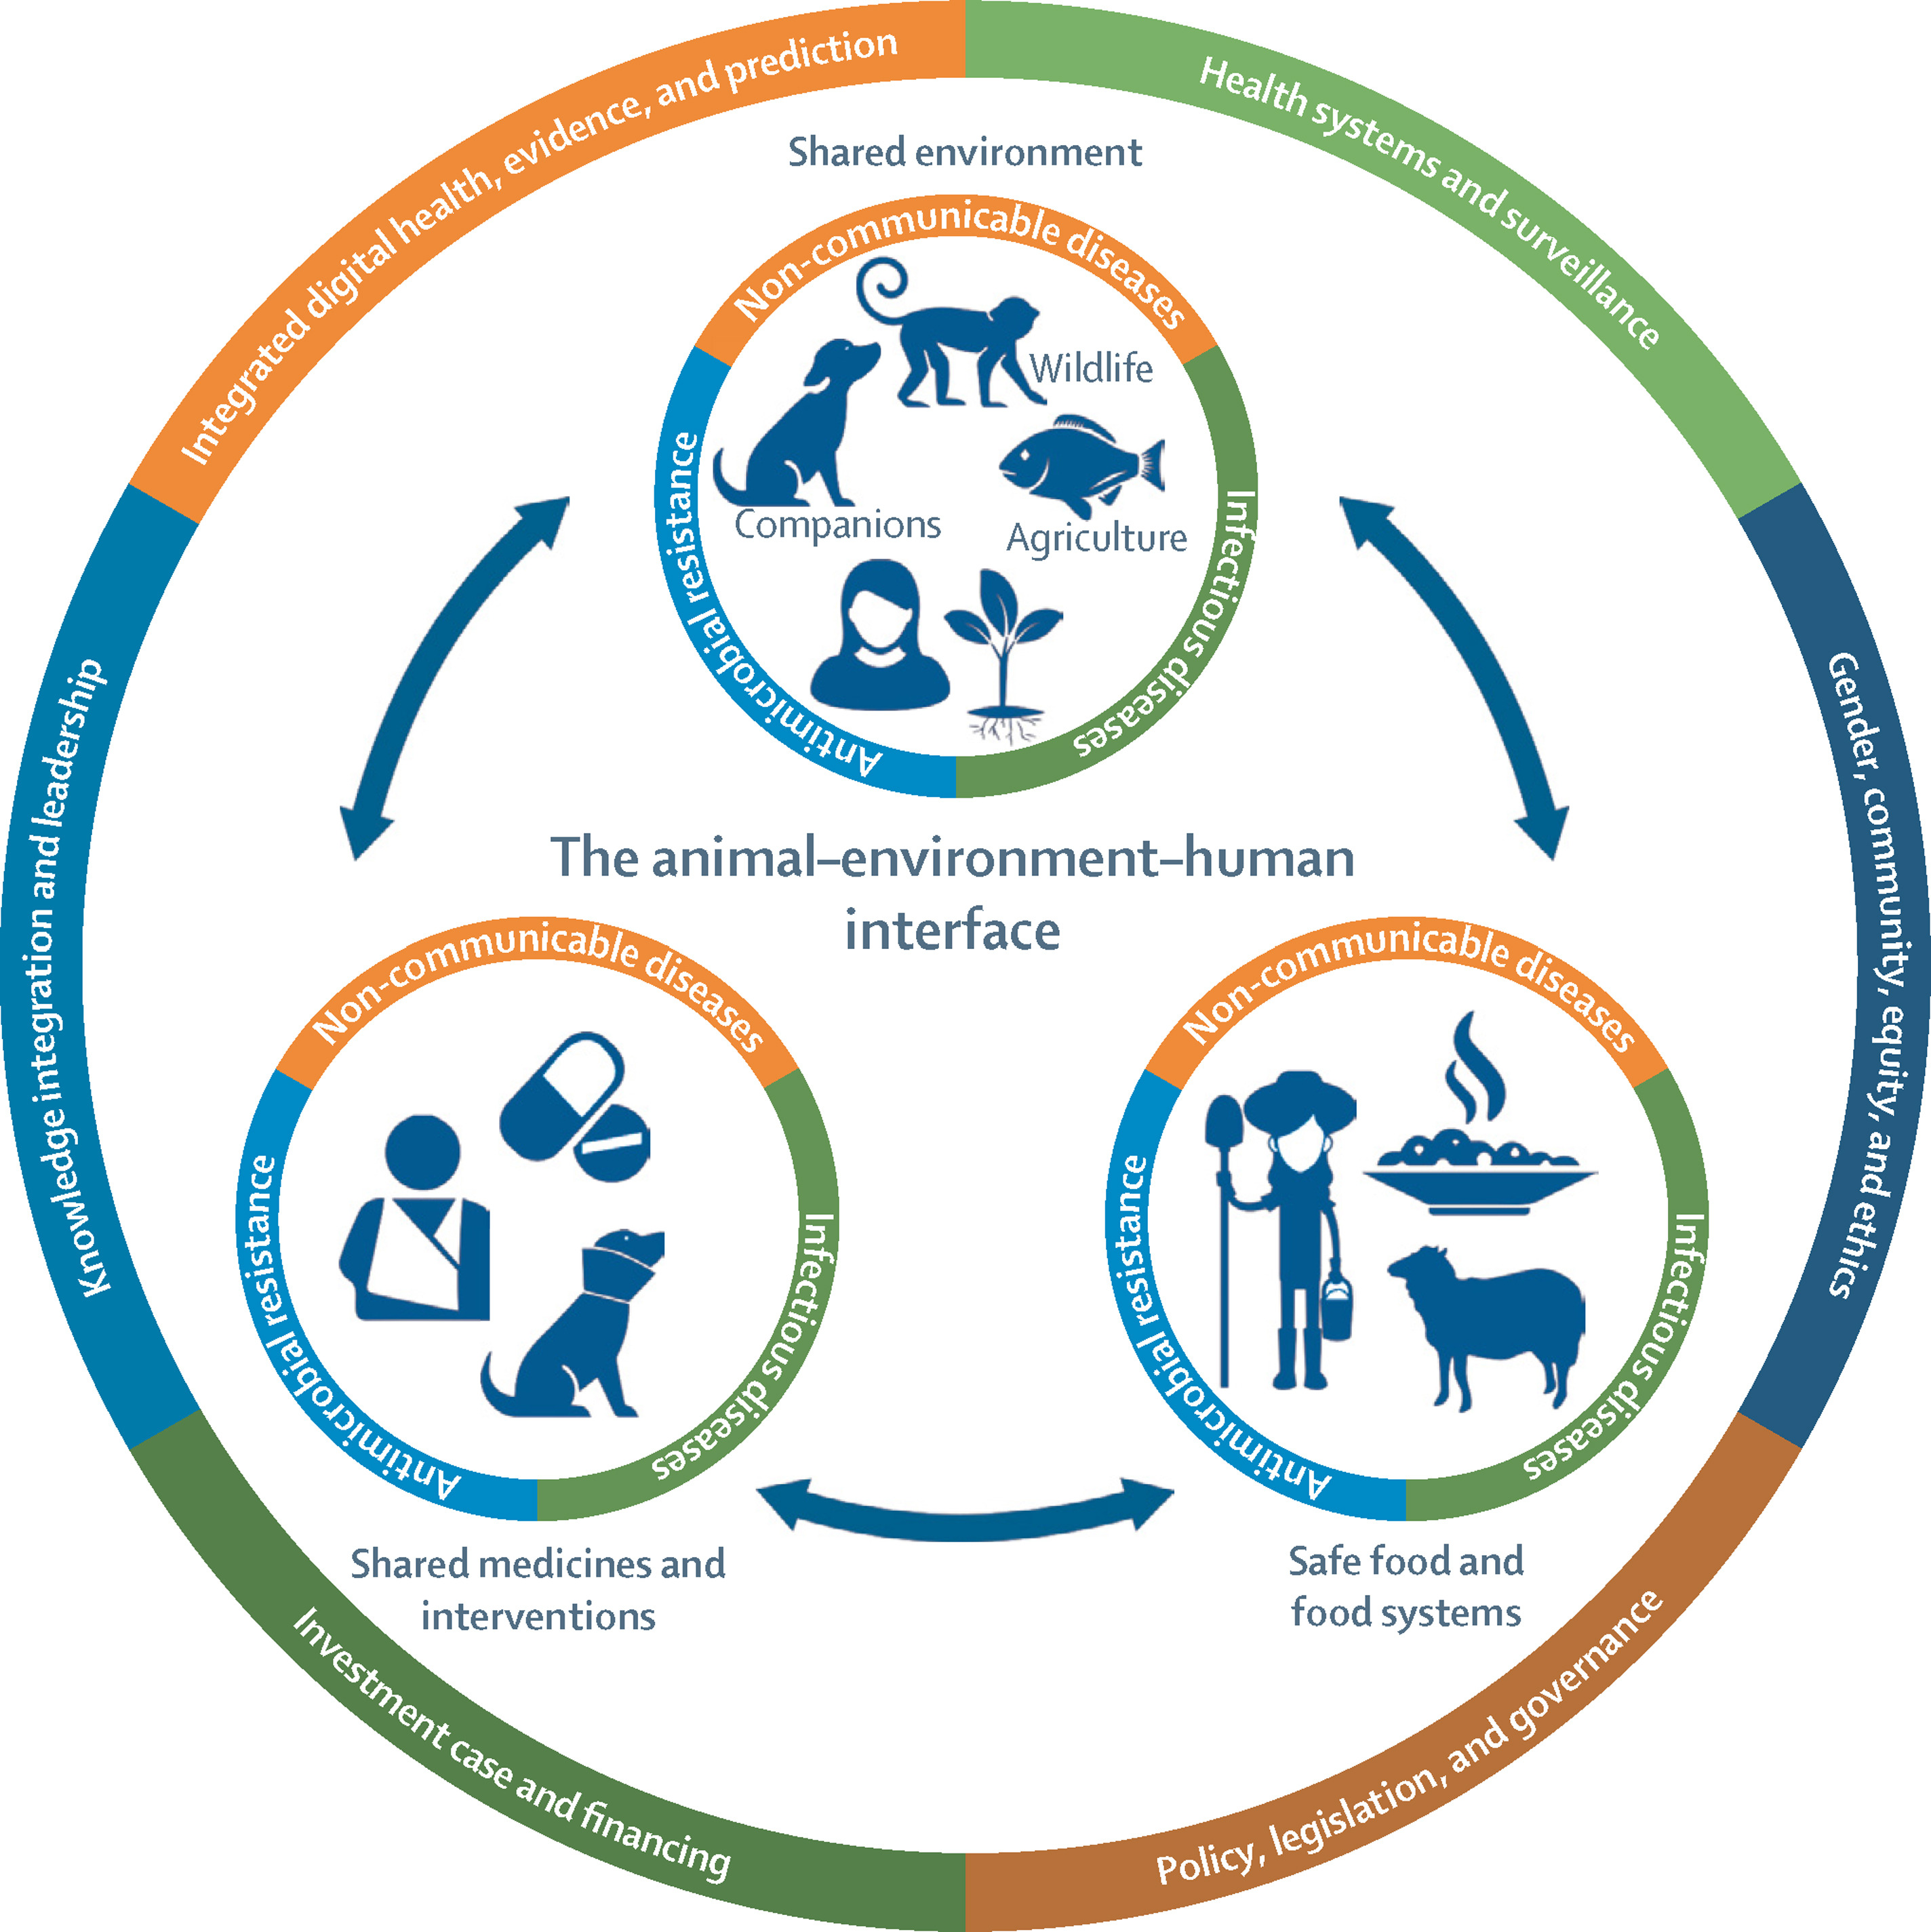
\includegraphics[height=\textheight]{FIGS/gr1_lrg.jpg}
% "https://doi.org/10.1016/S0140-6736(20)31027-8"
\end{frame}


\begin{frame}{Incidence \& Prevalence (when?)}
\defword{Incidence}: number of new cases in a population generated within a certain time period
\vfill
\defword{Prevalence}: number of cases of a disease at a single time point in a population
\vfill
$\implies$ $I(t)$ in an epidemiological model is \textbf{prevalence}, not \textbf{incidence}
\end{frame}

\begin{frame}{Exposition versus Exposed}
- Some bright bulb (not sure who) in days of yore: let's call \textbf{exposed} someone who has contracted the disease but is not yet showing symptoms ($\implies$ SEIR model)
\vfill
- "Real" epidemiologist: let's trace people who were exposed to the virus, i.e., people having come into contact with the virus (whether they have contracted the disease or not)
\vfill
- Interestingly, I have embarked on a quixotic quest to make people use $L$ instead of $E$, only to be told by real epidemiologists that they don't care \code{:)}
\end{frame}


\begin{frame}{Les différentes phases de la propagation}
- Spreading infectious disease: sporadic isolated cases
\vfill
- \defword{Outbreak}: the number of cases rises rapidly locally
\vfill
- \defword{Epidemic}: rapid rise and spread of an infectious disease in a given region
\vfill
- \defword{Endemic}: persistence habituelle d'une maladie infectieuse et contagieuse dans une région donnée
\vfill
- \defword{Pandemic}: épidémie qui s'étend au-delà des frontières des pays et qui peut se répandre sur un continent, un hémisphère ou dans le monde entier    
\end{frame}
        
\begin{frame}
        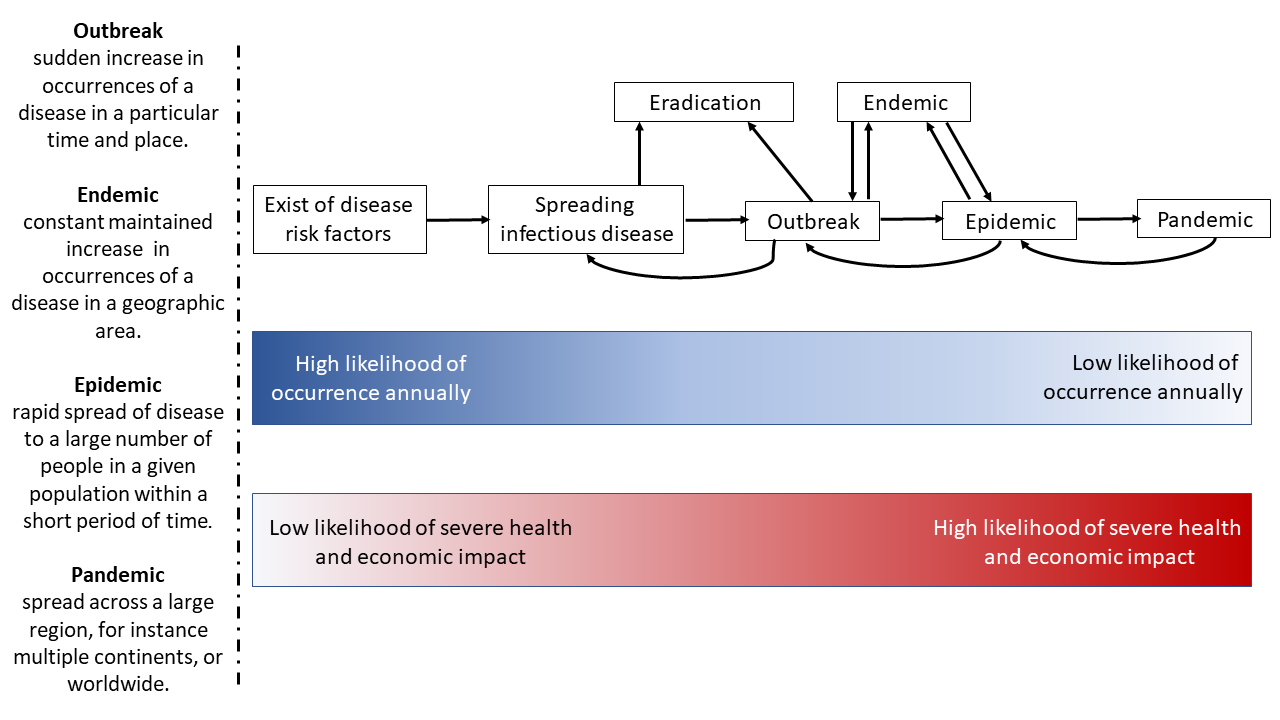
\includegraphics[width=\textwidth]{FIGS/Difference_between_outbreak,_endemic,_epidemic_and_pandemic-en.png}
\end{frame}
        


\begin{frame}{Epidemic curves}
- Used to record the occurrence of new cases as a function of time
\vfill
- When not too many cases, usually "individualised" (bar plots)
\vfill
- When number of cases is large, continuous curve
\end{frame}


\begin{frame}
    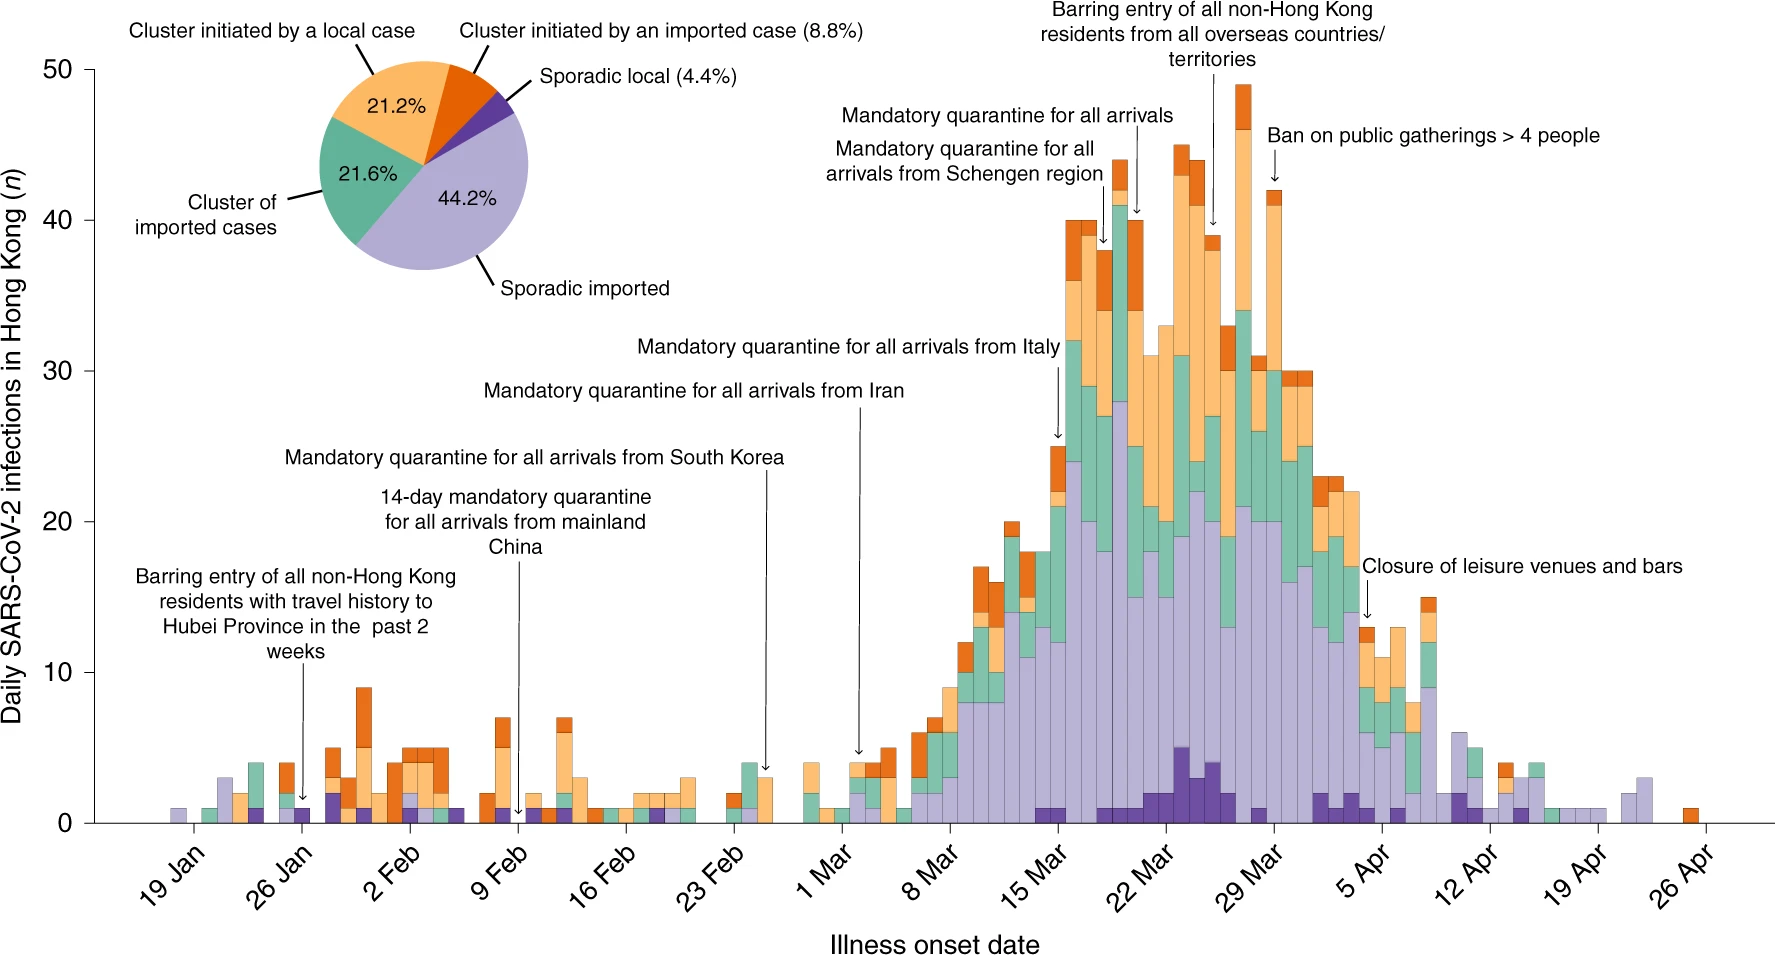
\includegraphics[width=\textwidth]{FIGS/41591_2020_1092_Fig1_HTML.png}
%"https://doi.org/10.1038/s41591-020-1092-0"
\end{frame}


\begin{frame}
    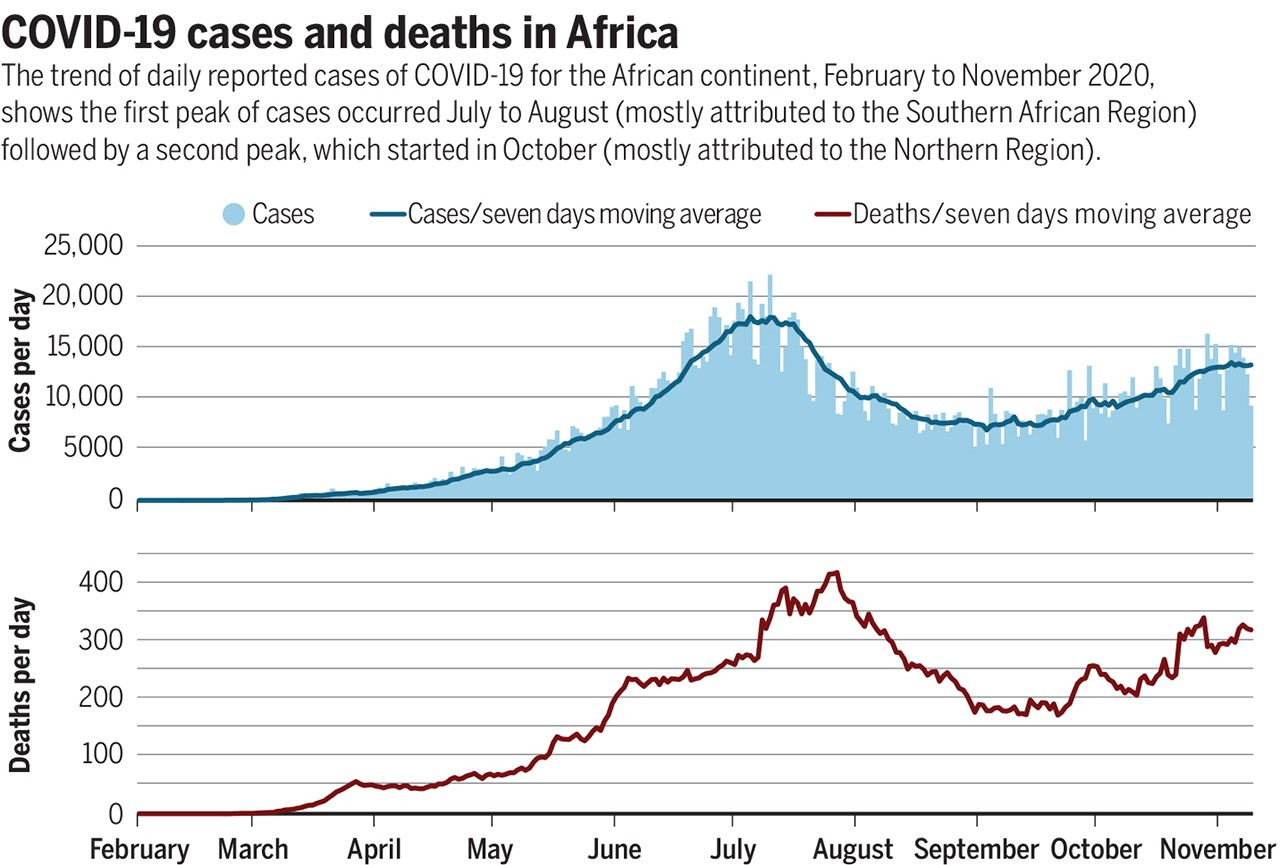
\includegraphics[width=\textwidth]{FIGS/371_27_f1.jpeg}
% "https://doi.org/10.1126/science.abf8832")
\end{frame}


\begin{frame}{Some terminology for ``where''}
- \defword{Epidemic}: diseases that are *visited upon* a population
\vfill
- \defword{Pandemic}: (will revisit this later in the course) epidemic that has spread across a large region, e.g., multiple continents or worldwide
\vfill
- \defword{Endemic}: diseases that *reside within* a population
\vfill
- We don't say "panendemic"
\end{frame}


\begin{frame}{Where? \href{https://en.wikipedia.org/wiki/1854_Broad_Street_cholera_outbreak}{1854 cholera outbreak}}
    \begin{minipage}{0.5\textwidth}
    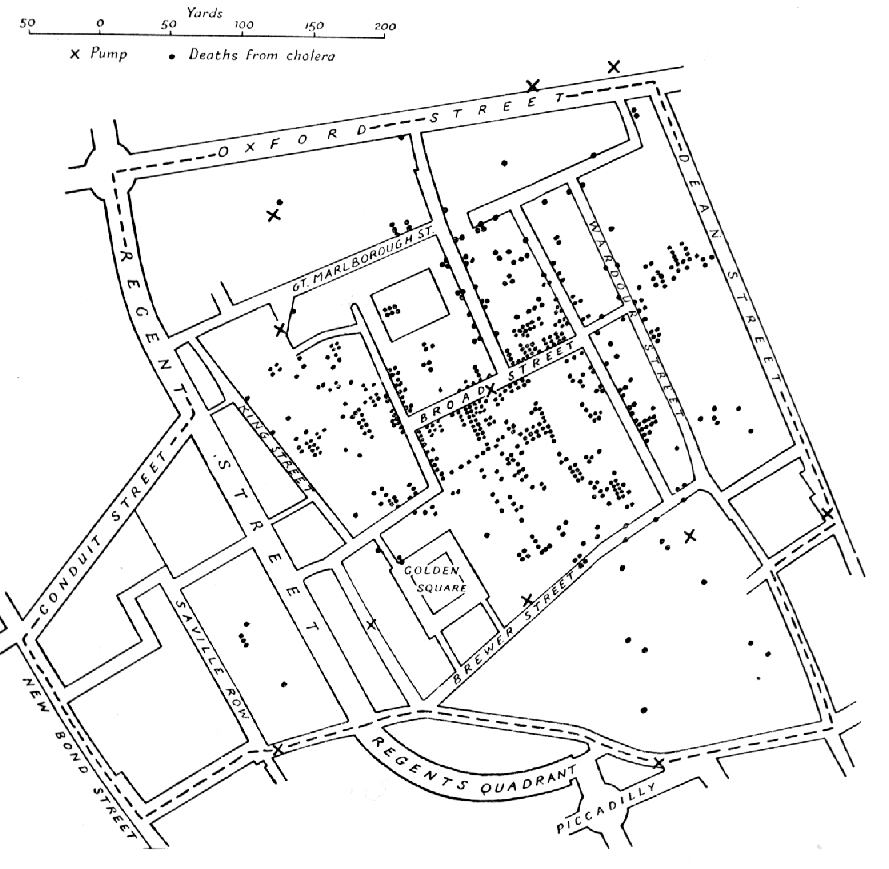
\includegraphics[width=\textwidth]{FIGS/Snow-cholera-map.jpg}
    \end{minipage}
    \begin{minipage}{0.45\textwidth}
        Cholera outbreak near Broad Street, London (UK)
        \vfill
        Studied by \href{https://en.wikipedia.org/wiki/John_Snow}{John Snow}

        \begin{quotation}
            I found that nearly all the deaths had taken place within a short distance of the [Broad Street] pump    
        \end{quotation}
            \end{minipage}
\end{frame}


\begin{frame}{\href{https://www.ncbi.nlm.nih.gov/books/NBK143061/}{WHO pandemic (influenza) phases}}
% <style>
%     .heatMap {
%         overflow:scroll;
%     }
%     .heatMap th {
%         background: grey;
%     }
%     .heatMap tr:nth-child(1) { background: green;}
%     .heatMap tr:nth-child(2) { background: green;}
%     .heatMap tr:nth-child(3) { background: yellow;}
%     .heatMap tr:nth-child(4) { background: yellow;}
%     .heatMap tr:nth-child(5) { background: orange;}
%     .heatMap tr:nth-child(6) { background: red;}
% </style>

% <div class="heatMap">

\begin{tabular}{ccp{6cm}}
Period & Phase & Description \\
\hline
\rowcolor{lgreen} \color{black}Interpandemic & \color{black}1 & \color{black} No animal influenza virus circulating among animals has been reported to cause infection in humans \\
\rowcolor{lgreen} & \color{black}2 & \color{black}Animal influenza virus circulating in domesticated or wild animals known to have caused infection in humans and therefore considered a specific potential pandemic threat
\end{tabular}
\end{frame}

\begin{frame}{\href{https://www.ncbi.nlm.nih.gov/books/NBK143061/}{WHO pandemic (influenza) phases}}
\begin{tabular}{ccp{6cm}}
Period & Phase & Description \\
\hline 
\rowcolor{yellow} \color{black}Pandemic alert & \color{black}3 & \color{black}Animal or human-animal influenza reassortant virus has caused sporadic cases or small clusters of disease in people, but has not resulted in H2H transmission sufficient to sustain community-level outbreaks \\
\rowcolor{yellow} & \color{black}4 & \color{black}Human-to-human transmission of an animal or human-animal influenza reassortant virus able to sustain community-level outbreaks has been verified 
\end{tabular}
\end{frame}

\begin{frame}{\href{https://www.ncbi.nlm.nih.gov/books/NBK143061/}{WHO pandemic (influenza) phases}}
\begin{tabular}{ccp{6cm}}
    Period & Phase & Description \\
    \hline 
\rowcolor{orange} \color{black}Pandemic alert & \color{black} 5 & \color{black} Same identified virus has caused sustained community-level outbreaks in at least 2 countries in 1 WHO region \\
\rowcolor{lred} \color{black}Pandemic & \color{black}6 & \color{black}In addition to criteria in Phase 5, same virus has caused sustained community-level outbreaks in at least 1 other country in another WHO region
\end{tabular}
\end{frame}

\begin{frame}
    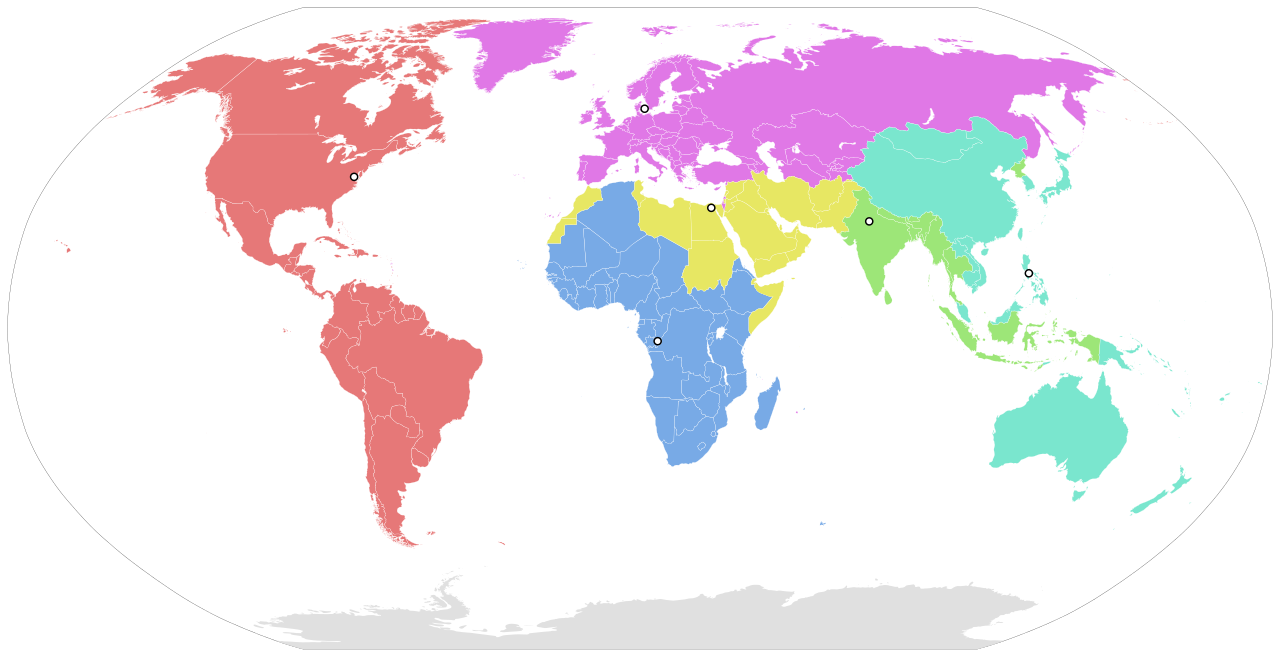
\includegraphics[width=\textwidth]{FIGS/1280px-World_Health_Organisation_regional_offices.png}
\end{frame}



%%%%%%%%%%%%%%%%%%%%
%%%%%%%%%%%%%%%%%%%%
\subsection{Fighting against infections}

\begin{frame}{Fighting against infections}
\begin{quote}
    Epidemiological information is used to plan and evaluate \defword{strategies to prevent illness} and as a guide to the \defword{management of patients} in whom disease has already developed  
\end{quote}
\vfill
- Preventing illness
\begin{itemize}
    \item Prophylactic measures
    \item Vaccination
\end{itemize}
\vfill
- Managing illness
\begin{itemize}
    \item Prevention of further spread (e.g., in hospital) 
    \item Treatment
\end{itemize}
\end{frame}


\begin{frame}{Immunisation}
- Smallpox first disease for which it was known 
\vfill
- Mentioned in a 1549 Chinese book
\vfill
- China: powdered smallpox scabs blown up noses of the healthy; variolation-induced mortality not negligible (0.5-2\%) but lower than normal (20\%)
\vfill
- 1798:  Edward Jenner introduces safer inoculation with cowpox (vaccination)
\vfill
- 1880s: Pasteur extends vaccination to chicken cholera and anthrax in animals and human rabies
\vfill
At the time, *herd immunity* was not understood so this was for personal protection
\end{frame}


\begin{frame}
<div style = "position: relative; top: -55%; padding-bottom:60px; font-size:40px">
Measles cases in the USA
</div>
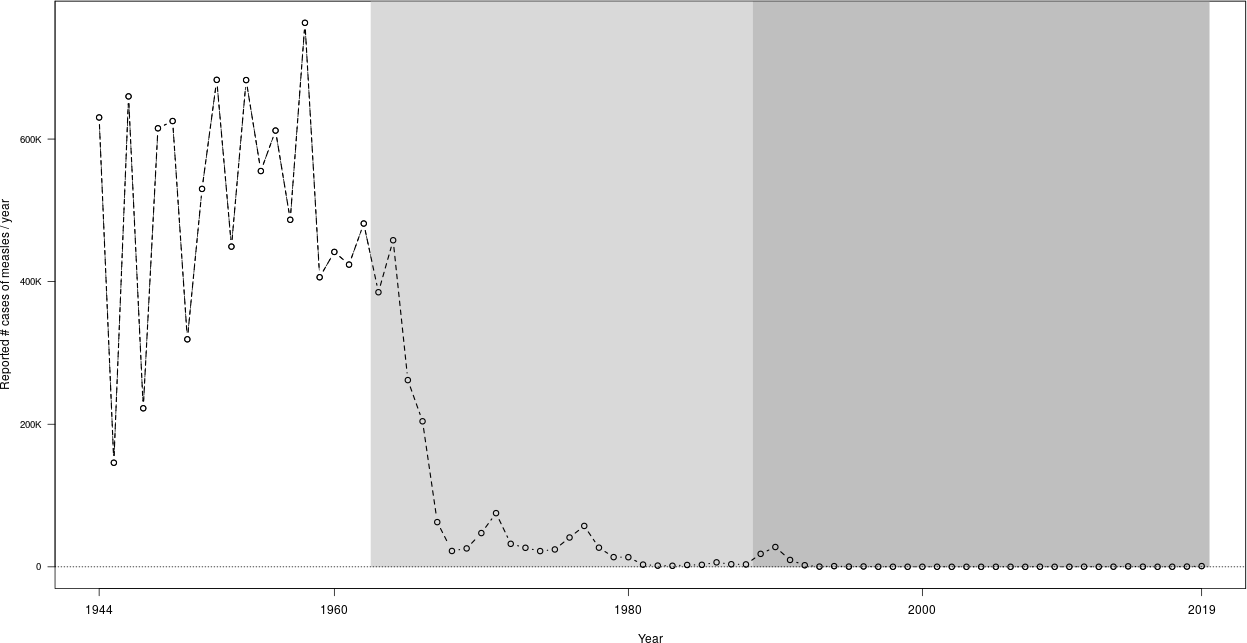
\includegraphics[width=\textwidth]{FIGS/measles_US_1944_2019.png}
\end{frame}


%%%%%%%%%%%%%%%%%%%%
%%%%%%%%%%%%%%%%%%%%
%%%%%%%%%%%%%%%%%%%%
%%%%%%%%%%%%%%%%%%%%
\section{Mathematical Epidemiology}

\begin{frame}{Domain is quite old ..}
.. but has only become a thing in recent years!
\end{frame}


\begin{frame}{Daniel Bernoulli (1760)}
\begin{minipage}{0.5\textwidth}
    
\includegraphics[width=\textwidth]{FIGS/Bernoulli-1760-first_page.jpg}
\end{minipage}
\begin{minipage}{0.47\textwidth}
\bbullet \href{https://gallica.bnf.fr/ark:/12148/bpt6k3558n/f220.item}{BNF scan} or \href{https://julien-arino.github.io/assets/pdf/Bernoulli-1760.pdf}{pdf}
\vfill
\bbullet Probably the first epidemic model
\vfill
\bbullet About petite vérole (smallpox) inoculation
\end{minipage}
\end{frame}


\begin{frame}{Ross (early 1900)}
\begin{minipage}{0.5\textwidth}
    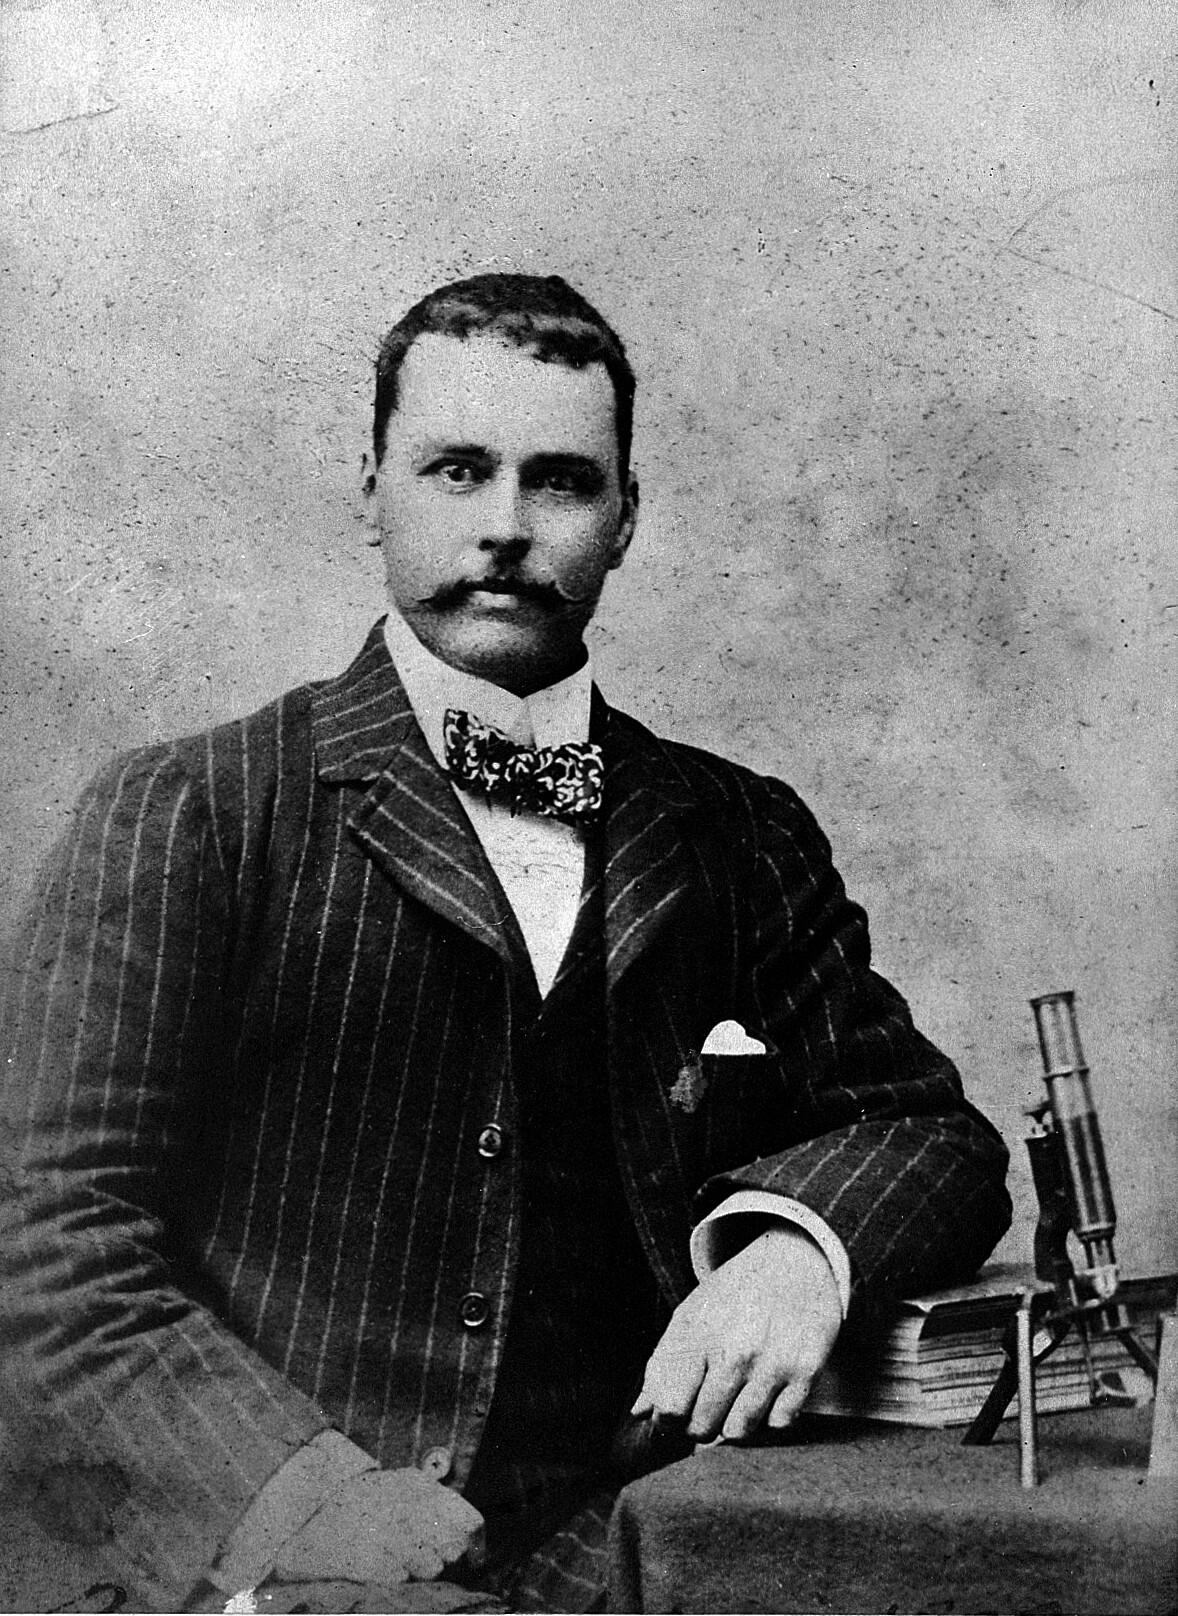
\includegraphics[width=\textwidth]{FIGS/RonaldRoss_WellcomeCollection.jpg}
\end{minipage}
\begin{minipage}{0.47\textwidth}
\bbullet On 20 August 1897, observed malaria parasites in the gut of a mosquito fed several days earlier on a malaria positive human
\vfill
\bbullet Nobel Prize for Medicine 1902
\vfill
\bbullet Started considering malaria eradication using mathematical models; for some history, read \href{https://www.ncbi.nlm.nih.gov/pmc/articles/PMC3320609/pdf/ppat.1002588.pdf}{this 2012 paper}
\end{minipage}
\end{frame}


\begin{frame}{Kermack and McKendrick (1927+)}
\bbullet We spend a lot more time on this in \href{https://julien-arino.github.io/3MC-course-epidemiological-modelling/2022_04_3MC_EpiModelling_L02_BasicMathEpi.html}{Lecture 05}
\vfill
\bbullet Groundbreaking set of papers starting in 1927
\vfill
\bbullet We will see one particular case, the most well known, but I point out here and point out in Lecture 05 that this is just the tip of the iceberg of their work
\end{frame}

\begin{frame}{Macdonald, Dietz and malaria}
\bbullet Read for instance \href{https://doi.org/10.1371/journal.ppat.1002588}{this paper}, which presents a history of the development of the so-called Ross-Macdonald model
\vfill
\bbullet Klaus Dietz also worked a lot on malaria
\end{frame}
    
    
\begin{frame}{Some activity later, but not much until 1990s}
\bbullet In recent years, explosion
\vfill
\bbullet Since the beginning of COVID-19: just nuts..
\end{frame}

\begin{frame}{Some landmarks in mathematical epidemiology (IMBO)}
\bbullet Macdonald. The epidemiology and control of malaria. 1957
\vfill
\bbullet Baroyan, Rvachev et al. Deterministic epidemic models for a territory with a transport network. Kibernetika, 1967
\vfill
\bbullet Hethcote \& Yorke. Gonorrhea Transmission Dynamics and Control. LNBM 56, 1984
\vfill
\bbullet Anderson \& May. Infectious diseases of humans: dynamics and control. 1991
\vfill
\bbullet Capasso. Mathematical Structures of Epidemic Systems. LNBM 97, 1993
\vfill
\bbullet Hethcote. The mathematics of infectious diseases. SIAM Review, 2000
\vfill
\bbullet van den Driessche \& Watmough. Reproduction numbers and sub-threshold endemic equilibria for compartmental models of disease transmission. MBS, 2002      
\end{frame}


%%%%%%%%%%%%%%%%%%%%
%%%%%%%%%%%%%%%%%%%%
\subsection{Computational epidemiology}

\begin{frame}{A more recent trend}
- Some rare numerical work $\leq$ 1980s, mostly simulation of math models
\begin{itemize}
    \item Baroyan, Rvachev et al. \href{https://doi.org/10.2307/1426167}{Computer modelling of influenza epidemics for the whole country (USSR)}. \emph{Advances in Applied Probability} (1971) 
    \item Rvachev \& Longini. \href{https://doi.org/10.1016/0025-5564(85)90064-1}{A mathematical model for the global spread of influenza}. \emph{Mathematical Biosciences} (1986) 
    \item Flahault, Letrait et al. \href{https://doi.org/10.1002/sim.4780071107}{Modelling the 1985 influenza epidemic in France}. \emph{Statistics in Medicine} (1988)
\end{itemize}
\vfill
- More and more frequent now, to the point that some modelling studies are purely simulation-based
\end{frame}

\begin{frame}{Agent-based models (ABM)}
\bbullet Early in the life of these models, they were called IBM (individual-based models)
\vfill
\bbullet Over the years, a "philosophical" distinction has emerged:
\begin{itemize}
\item IBM are mathematical models that consider individuals as the units; e.g., DTMC, CTMC, branching processes, etc.
\item ABM are computational models whose study is, for the most part, only possible numerically 
\end{itemize}
\end{frame}

\begin{frame}{Network models}
\bbullet Network models endow vertices with simple systems and couple them through graphs
\vfill
\bbullet Can be ABM, but some networks can also be studied analytically

\end{frame}

%%%%%%%%%%%%%%%%%%%%
%%%%%%%%%%%%%%%%%%%%
\subsection{Use of data in epidemiology}

\begin{frame}{Has happened all along, undergoing a transformation}
\bbullet Epidemiology has long relied on data
\vfill
\bbullet Many developments in statistics originate there
\vfill
\bbullet Data has traditionally been better for chronic diseases than for infectious ones
\vfill
\bbullet Near-real-time surveillance of infectious diseases ongoing since the 1980s (e.g., Réseau Sentinelles)
\vfill
\bbullet SARS-CoV-1 saw the beginning of a move towards real-time emerging infectious disease data
\vfill
\bbullet With SARS-CoV-2, the system has really progressed a lot, both in terms of "citizen science" and governmental initiatives
\end{frame}






\end{document}
